\documentclass[letterpaper,10pt]{article}

%\setlength{\parindent}{0in}
%\usepackage{fullpage} 
\usepackage{amsmath}
\usepackage{amssymb}
\usepackage{enumerate}
\usepackage{graphicx}
\usepackage{dcolumn}
\oddsidemargin 0.0in
\textwidth 6.5in
\newcolumntype{.}{D{.}{.}{-1}}
\newcommand{\Mct}{\overline{\mbox{M}}\mbox{ct}}

%opening
\title{Assignment 3}
\author{Steve Mazza}
\date{October 21, 2011}

% Complete problems 13.1, 13.4, 13.5, 13.8, 13.11, and 13.12 from B&F.
\begin{document}
\maketitle

\begin{description}
\item[13.1]\ \emph{Maintainability} is a characteristic, or result, of design that is expressed in terms of different measures of \emph{maintenance,} activities performed pursuant to sustainment of proper system function.  Maintainability (an attribute) drives maintenance (an activity).

\item[13.4]\ MTBF is the average time between failures (unscheduled) whereas MTBM is the average time between all maintenance actions (both corrective and preventative).  MTBR is the average time between item replacement as a result of either corrective or preventative maintenance.  MTBR is a factor of MTBM.

\item[13.5]
\begin{enumerate}[(a)]
\item The range of observations is between 11 and 47.
\item Using a class interval width of 4 yields 10 class intervals.  The distribution looks \emph{lognormal}.
\begin{center}
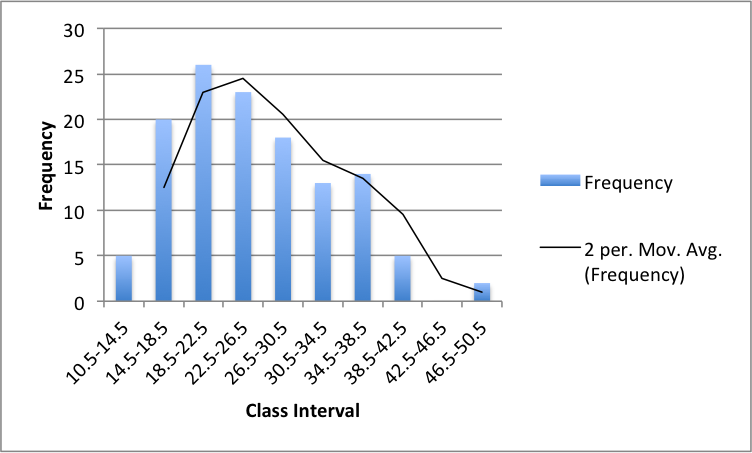
\includegraphics[scale=0.75]{assignment3mazzaImage0.png}
\end{center}
\item $\Mct = 27.7\overline{22}$.
\item The geometric mean of the repair times is 25.67330796.
\item The standard deviation of the sample data is 10.42511422.
\item M$_{\mbox{max}} =6.533504415$.
\end{enumerate}

\item[13.8]\ I had some problems here because it looks like ``Mean logistics plus administrative'' is \emph{Given} however no value is supplied.  It greatly helps if I assume the value to be 0 although I admit this to be a leap of faith.  Please see the accompanying spreadsheet for calculations. \\
\begin{align*}
A_{i} &= 0.803858521 \\
A_{a} &= 0.689655172 \\
A_{o} &= 0.689655172 \\
\Mct &= 61 \\
M_{max} &= n/a \\
MTBM &= 111.\overline{11} \\
MTBF &= 250 \\
\overline{M} &= 50 \\
MTTR_{g} &= n/a
\end{align*}

\item[13.11]\ Please see the accompanying spreadsheet for calculations. \\
\begin{table}[htdp]
\begin{center}
\begin{tabular}{ccc..c.}
\hline
Assembly & Quantity & $\lambda$ & C$$_{f}$$ & C$$_{p}$$ & $\Mct$ & C$$_{t}$$ \\
\hline 
A & 1 & 0.05 & 0.05 & 0.065789474 & 1.3 & 0.065 \\
B & 2 & 0.16 & 0.32 & 0.421052632 & 1.0 & 0.32 \\
C & 1 & 0.27 & 0.27 & 0.355263158 & 0.9 & 0.243 \\
D & 1 & 0.12 & 0.12 & 0.157894737 & 1.1 & 0.132 \\
\hline
& & & 0.76 & 1 & & 0.76
\end{tabular}
\end{center}
\label{default}
\end{table}%
$\Mct \mbox{\ for System\ } ABCD = \frac{\sum C_{t}}{\sum C_{f}} = \frac{0.76}{0.76} = 1$.

\item[13.12]\ MLH/OH = 0.01 for the parameters given.  Please see the accompanying spreadsheet for calculation.

\end {description}
\end{document}